%%%%%%Experiments%%%%%%%%

\begin{table*}[!t]
  \centering
  \caption{\small{Comparison of VQ-VAEs trained on ImageNet dataset following~\citep{Oord2017NeuralDR}.}}
  \label{tab:vqvae imagenet}
  \vspace{-2ex}
  \resizebox{0.82\textwidth}{!}{%
  \begin{tabular}{lcccccccc} \hline
    Approaches & Tokens & Codebook Size & $\mathcal{U}$ ($\uparrow$) & $\mathcal{C}$ ($\uparrow$) & PSNR($\uparrow$) & SSIM($\uparrow$) & Rec. Loss ($\downarrow$) \\\hline
    Vanilla VQ & 256 & $16384$ & 2.5\% & 360.7 & 24.44 & 57.5 & 0.0294 \\ 				
    STE++ & 256 & $16384$ & 6.5\% & 889.9 & 24.88 & 58.9 & 0.0270\\
    EMA VQ & 256 & $16384$ & 14.5\% & 1861.5 & 24.98 & 59.2 & 0.0267  \\
    Online VQ & 256 & $16384$ & 22.2\% & 1465.6 & 24.88 & 58.6 & 0.0273 \\
    \textbf{Wasserstein VQ} & 256 & $16384$ & \textbf{100\%} & \textbf{15539.1} & \textbf{25.47} & \textbf{61.2} & \textbf{0.0242} \\\hline
    Vanilla VQ  & 256 & $50000$ & 0.9\% & 378.7 & 24.40 & 57.7 & 0.0295 \\ 				
    STE++ & 256 & $50000$ & 2.0\% & 851.7 & 24.89 & 59.0 & 0.0270\\
    EMA VQ  & 256 & $50000$ & 16.8\% & 6139.3 & 25.37 & 60.9 & 0.0246 \\
    Online VQ & 256 & $50000$ & 9.9\% & 2241.7 & 25.09 & 59.7 & 0.0260  \\
    \textbf{Wasserstein VQ} & 256 & $50000$ & \textbf{100\%} & \textbf{46133.2} & \textbf{25.72} & \textbf{62.3} & \textbf{0.0230} \\\hline
    Vanilla VQ & 256 & $100000$  & 0.4\% & 337.0 & 24.43 & 57.4 & 0.0295 \\ 				
    STE++ & 256 & $100000$ & 0.9\% & 730.6 & 24.86 & 59.1 & 0.0269\\
    EMA VQ  & 256 & $100000$ & 3.0\% & 2170.0 & 25.13 & 60.1 & 0.0257\\
    Online VQ  & 256 & $100000$ & 4.1\% & 1709.9 & 24.95 & 59.1 & 0.0267  \\
    \textbf{Wasserstein VQ} & 256 & $100000$ & \textbf{100\%} & \textbf{93264.7} & \textbf{25.88} & \textbf{63.0} & \textbf{0.0223} \\\hline
    \vspace{-0.4cm}
  \end{tabular}
}
\vspace{-2ex}
\end{table*}



\section{Experiments}\label{sec:experiments}

In this section, we empirically demonstrate the effectiveness of \emph{Wasserstein VQ} in visual tokenization tasks. Experiments are conducted within the VQ-VAE~\citep{Oord2017NeuralDR} and VQGAN~\citep{Esser2020TamingTF} frameworks. PyTorch code, including training environments, scripts, and logs, will be made publicly available.

\subsection{Evaluation on VQ-VAE Framework}
\label{sec:vqvae experiments}
\paragraph{Datasets and Baselines.} Experiments are conducted on four benchmark datasets: two low-resolution datasets, i.e., CIFAR-10~\citep{Krizhevsky2009LearningML} and SVHN~\citep{Netzer2011ReadingDI},  and two high-resolution datasets FFHQ~\citep{Karras2018ASG} and ImageNet~\citep{Deng2009ImageNetAL}. We evaluate our approach against representative VQ methods:  Vanilla VQ~\citep{Oord2017NeuralDR}, EMA VQ~\citep{Razavi2019GeneratingDH}, which uses exponential moving average updates and is also referred to as $k$-means, Online VQ, which employs $k$-means++ in CVQ-VAE~\citep{Zheng2023OnlineCC}, and enhanced  straight-through estimator STE++~\citep{Huh2023StraighteningOT}. For experimental settings, see Appendix~\ref{appendix:experimental details}. 
\vspace{-2ex}

\paragraph{Metrics.}
We employ multiple evaluation metrics, including the codebook utilization rate ($\mathcal{U}$), codebook perplexity ($\mathcal{C}$), peak signal-to-noise ratio (PSNR), patch-level structural similarity index (SSIM), and pixel-level reconstruction loss (Rec. Loss). We exclude quantization error ($\mathcal{E}$) from the reported results, as it is highly sensitive to variances—a factor analyzed in Appendix~\ref{appendix:Impact of Distribution Variance}. Since these variances remain uncontrolled in our experiments, comparison based on 
($\mathcal{E}$) would be unreliable. To ensure an equitable assessment, Appendix~\ref{appendix:discussion} provides an atomic setting where distribution variances are controlled and identical across all VQ variants.
\vspace{-2ex}

\paragraph{Main Results.} 
As shown in Table~\ref{tab:vqvae imagenet}, and Table~\ref{tab:vqvae ffhq},~\ref{tab:vqvae cifar10},~\ref{tab:vqvae svhn} in the Appendix~\ref{appendix:vqvae cifar-10 and svhn}, our proposed \emph{Wasserstein VQ} outperforms all baselines across datasets, achieving superior performance on almost all evaluation metrics under various settings. This is because VQ inherently functions as a compressor, mapping a continuous latent space to a discrete one, where minimal information loss indicates improved expressivity. Our \emph{Wasserstein VQ} employs explicit distribution matching constraints, achieving improved alignment between feature and code vectors. This yields nearly 100\% codebook utilization and near-minimal quantization error, resulting in the lowest reconstruction loss.

\begin{table*}[!t]
\vspace*{-10pt}
\centering
\caption{
    {Reconstruction performance on the ImageNet-1K dataset. The suffixes “–a,” “–b,” and “–c” correspond to decoder adaptation for 5, 10, and 15 epochs, respectively. The best-performing result is highlighted in bold. Results marked with $^{\dagger}$ are cited from VQGAN-LC \citep{Zhu2024ScalingTC}, those with $^{\star}$ from Llama GEN \citep{Sun2024AutoregressiveMB}, and those with $^{\ddagger}$ from VQ-Transplant \citep{Fang2025VQTransplant}. }
    }
\vspace*{-10pt}
\resizebox{0.85\textwidth}{!}{
\begin{tabular}{lcccccccc}
\toprule
Methods & Tokens  & Codebook Size $K$ & $\mathcal{U}$ ($\uparrow$) & r-FID $\downarrow$ & r-IS $\uparrow$ & LPIPS $\downarrow$ & PSNR $\uparrow$ & SSIM $\uparrow$\\
\midrule
DQVAE$^{\dagger}$ & 256  & 1024 & - & 4.08  & - & - & - & - \\
DiVAE$^{\dagger}$ & 256 & 16384 & - & 4.07 & - & - & - & - \\
RQVAE$^{\dagger}$ & 256 & 16384 & - &  3.20 & - & - & - & -\\
RQVAE$^{\dagger}$ & 512 & 16384 & - & 2.69 & - & - & - & -\\
RQVAE$^{\dagger}$ & 1024 & 16384 & - & 1.83 & - & - & -  & -\\
DF-VQGAN$^{\dagger}$ & 256 & 12288 & - & 5.16 & - & - & - & - \\
DF-VQGAN$^{\dagger}$ & 1024 & 8192 & - & 1.38 & - & - & - & - \\
Llama GEN$^{\star}$ & 256 & 16384 & 97.0\% & 2.19 & -  & - &  20.79 & 67.5 \\
\midrule
\multirow{3}{*}{VQGAN$^{\dagger}$}  & 256 & 16384 & 3.4\% & 5.96 & - & 0.17 & 23.3& 52.4 \\
& 256 &  50000 & 1.1\% & 5.44 & - & 0.17 & 22.5 & 52.5 \\
& 256 &  100000 & 0.5\% &  5.44 & - & 0.17 & 22.3 & 52.5 \\
\midrule
\multirow{3}{*}{VQGAN-FC$^{\dagger}$} & 256 & 16384 & 11.2\%  & 4.29 & - & 0.17 & 22.8 & 54.5 \\ 
& 256 & 50000 & 3.6\%  & 4.96 & - & 0.15 & 23.1 & 54.7 \\
& 256 & 100000 & 1.9\%  & 4.65 & - & 0.15 & 22.9 & 55.1 \\
\midrule
\multirow{3}{*}{VQGAN-EMA$^{\dagger}$} & 256 & 16384 & 83.2\% & 3.41 & -  & 0.14 & 23.5 & 56.6 \\
& 256 & 50000 &  40.2\% & 3.88 & -  & 0.14 & 23.2 & 55.9 \\
& 256 & 100000 & 24.2\% & 3.46 & -  &  0.13 & 23.4 & 56.2 \\
\midrule
\multirow{4}{*}{VQGAN-LC$^{\dagger}$} & 256 & 16384 & \textbf{99.9\%}  & 3.01 & - & 0.13 & 23.2 & 56.4 \\
 & 256 & 50000 & \textbf{99.9\%}  & 2.75 & - & 0.13 &  23.8 &  58.4 \\
 & 256 & 100000 & \textbf{99.9\%}  & 2.62 & - &  0.12 &  23.8 & 58.9 \\
 & 1024 & 100000 & 99.5\%  & 1.29 & - &  \textbf{0.07} &  \textbf{27.0} &  \textbf{71.6} \\\midrule
\midrule
\multirow{3}{*}{\textbf{Wasserstein VQ-a}$^{\ddagger}$} & 512 & 16384 & 99.8\% & 1.04 & 191.3 & 0.114 & 24.36 & 64.0 \\
& 512 & 32768 &  99.7\% & 0.98 &  193.9 & 0.111 & 24.37 & 64.3 \\
& 512 & 65536 & 99.6\% & 0.92 & 195.5 & 0.106 & 24.68 & 65.4 \\\midrule
\multirow{3}{*}{\textbf{Wasserstein VQ-b}} & 512 & 16384 & 99.8\% & 0.98 & 192.9 & 0.114 & 24.34 & 63.7\\
& 512 & 32768 & 99.8\% & 0.88 & 196.2 & 0.109 & 24.60 & 64.7 \\
& 512 & 65536 & 99.6\% & 0.81 & \textbf{198.7} & 0.105 & \textbf{24.77} & \textbf{65.5}\\\midrule
\multirow{3}{*}{\textbf{Wasserstein VQ-c}} & 512 & 16384 & 99.8\% & 0.90 & 194.1 & 0.114 & 24.27 & 63.4\\
& 512 & 32768 & 99.8\% & 0.85 & 196.4 & 0.109 & 24.43 & 64.1 \\
& 512 & 65536 & 99.6\% & \textbf{0.79} & 198.5 & \textbf{0.104} & 24.73 & 65.2 \\
\bottomrule
\end{tabular}}
\vspace{-2ex}
\label{tab:reconstruction_IN-main table}
\end{table*}

\begin{table}[!t]
\centering
\caption{
    {Reconstruction performance on the ImageNet-1K dataset for multi-scale quantization algorithms. The suffixes “–a,” “–b,” and “–c” correspond to decoder adaptation for 5, 10, and 15 epochs, respectively. For each codebook size, the best-performing result is highlighted in bold. $^{\ddagger}$: results are cited from VQ-Transplant \citep{Fang2025VQTransplant}. }
    }
\vspace*{-10pt}
\resizebox{0.48\textwidth}{!}{
\begin{tabular}{lcccccccc}
\toprule
Methods & Tokens  & Codebook Size $K$ & $\mathcal{E}$ ($\downarrow$) & $\mathcal{U}$ ($\uparrow$) & $\mathcal{C}$ ($\uparrow$) & r-FID $\downarrow$ \\\midrule
VAR$^{\ddagger}$ & 680 & 4096 & 0.283 & \textbf{100\%} & 2981.4 & 0.92\\\midrule
\multirow{2}{*}{Vanilla VAR$^{\ddagger}$} & 680 & 4096 & 0.305 & 38.2\% & 1300.4 & 1.25 \\
& 680 & 8192 & 0.309 & 22.9\% & 1422.6 & 1.30\\\midrule
\multirow{2}{*}{EMA VAR$^{\ddagger}$} & 680 & 4096 & 0.321 & 99.9\% & 1806.6 &  1.69 \\
& 680 & 8192 &  0.312 & 99.8\% & 2498.8 &  1.15\\\midrule
\multirow{2}{*}{Online VAR$^{\ddagger}$} & 680 & 4096 &  0.276 &  99.0\% & 1950.9 & 1.05\\
& 680 & 8192 & 0.269 & 73.9\% & 3588.6 & 1.00\\\midrule
\multirow{2}{*}{\textbf{Wasserstein VAR-a}$^{\ddagger}$} & 680 & 4096 & \textbf{0.255} & \textbf{100\%} &  \textbf{3286.2} & 0.93 \\
& 680 & 8192 &  \textbf{0.240}  & \textbf{100\%} & \textbf{6518.2}
 & 0.83\\\midrule
\multirow{2}{*}{\textbf{Wasserstein VAR-b}} & 680 & 4096 & \textbf{0.255} & \textbf{100\%} & \textbf{3286.2} & 0.88 \\
& 680 & 8192 &  \textbf{0.240}  & \textbf{100\%} & \textbf{6518.2}
 & 0.79 \\\midrule
\multirow{2}{*}{\textbf{Wasserstein VAR-c}} & 680 & 4096 & \textbf{0.255} & \textbf{100\%} & \textbf{3286.2} & \textbf{0.81} \\
& 680 & 8192 &  \textbf{0.240}  & \textbf{100\%} & \textbf{6518.2}
 & \textbf{0.73}\\
\bottomrule
\end{tabular}}
\vspace{-4ex}
\label{tab:reconstruction_IN-multi-scale}
\end{table}

% \begin{figure}[!t]
% \begin{center}
%     \vspace{-1mm}
%     \subfloat[\small{Feature Density}]{ 
%     \label{fig:density}  
%     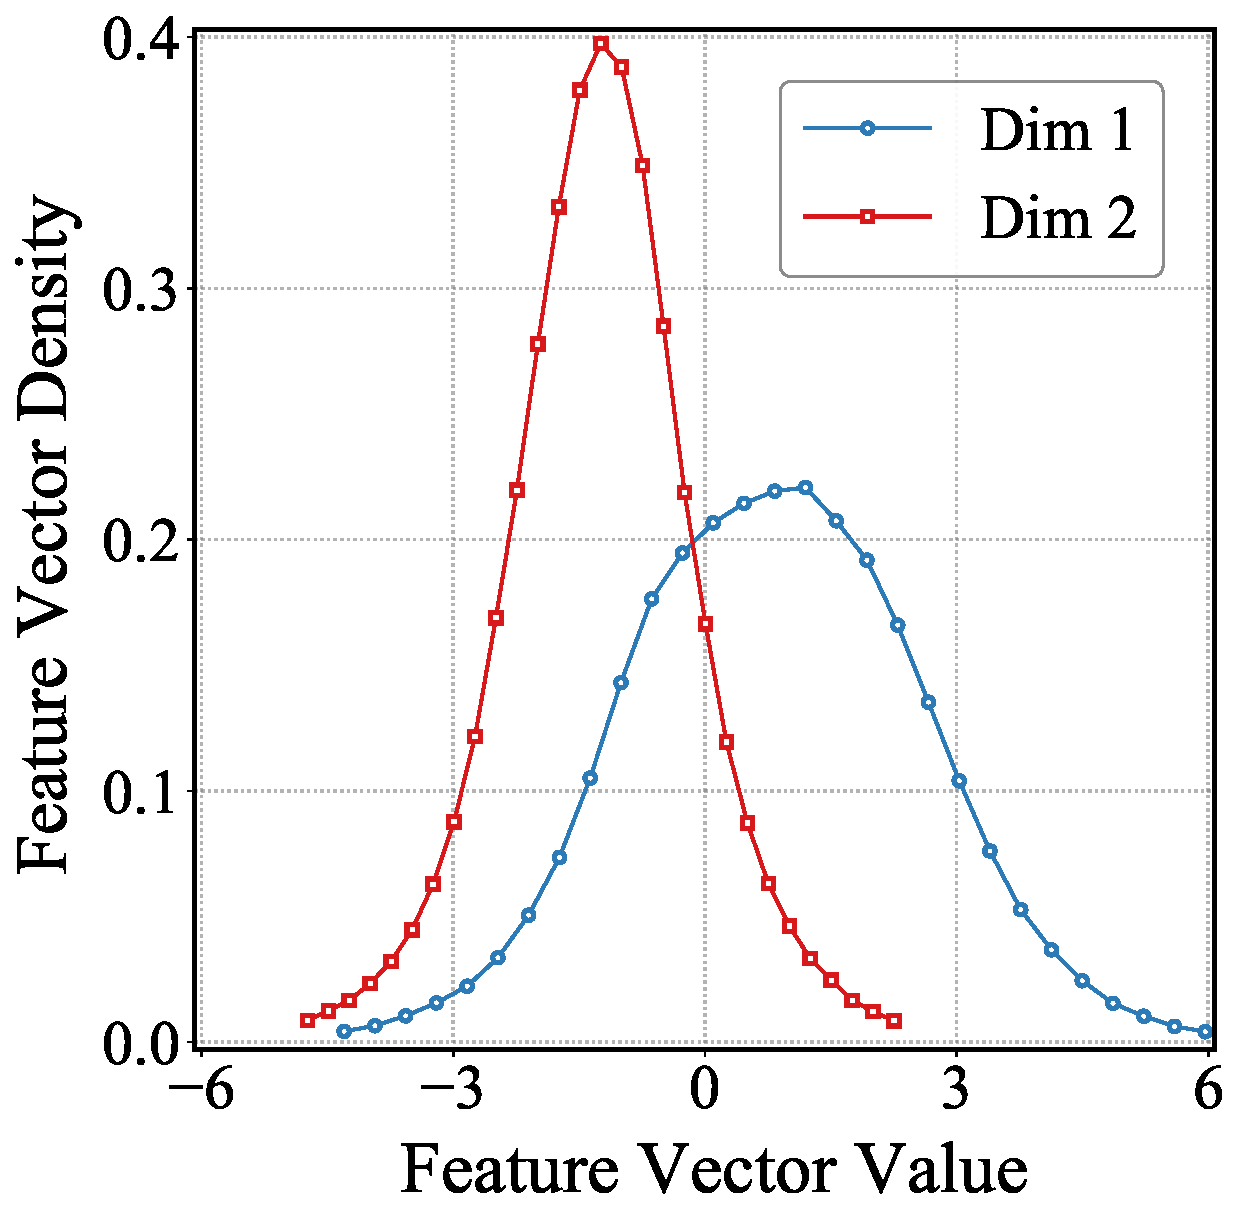
\includegraphics[width=0.24\textwidth]         {figs/Gaussion/feature_density.pdf}}
%     \subfloat[\small{Feature Visualization}]{
%     \label{fig:feature visualization}
%     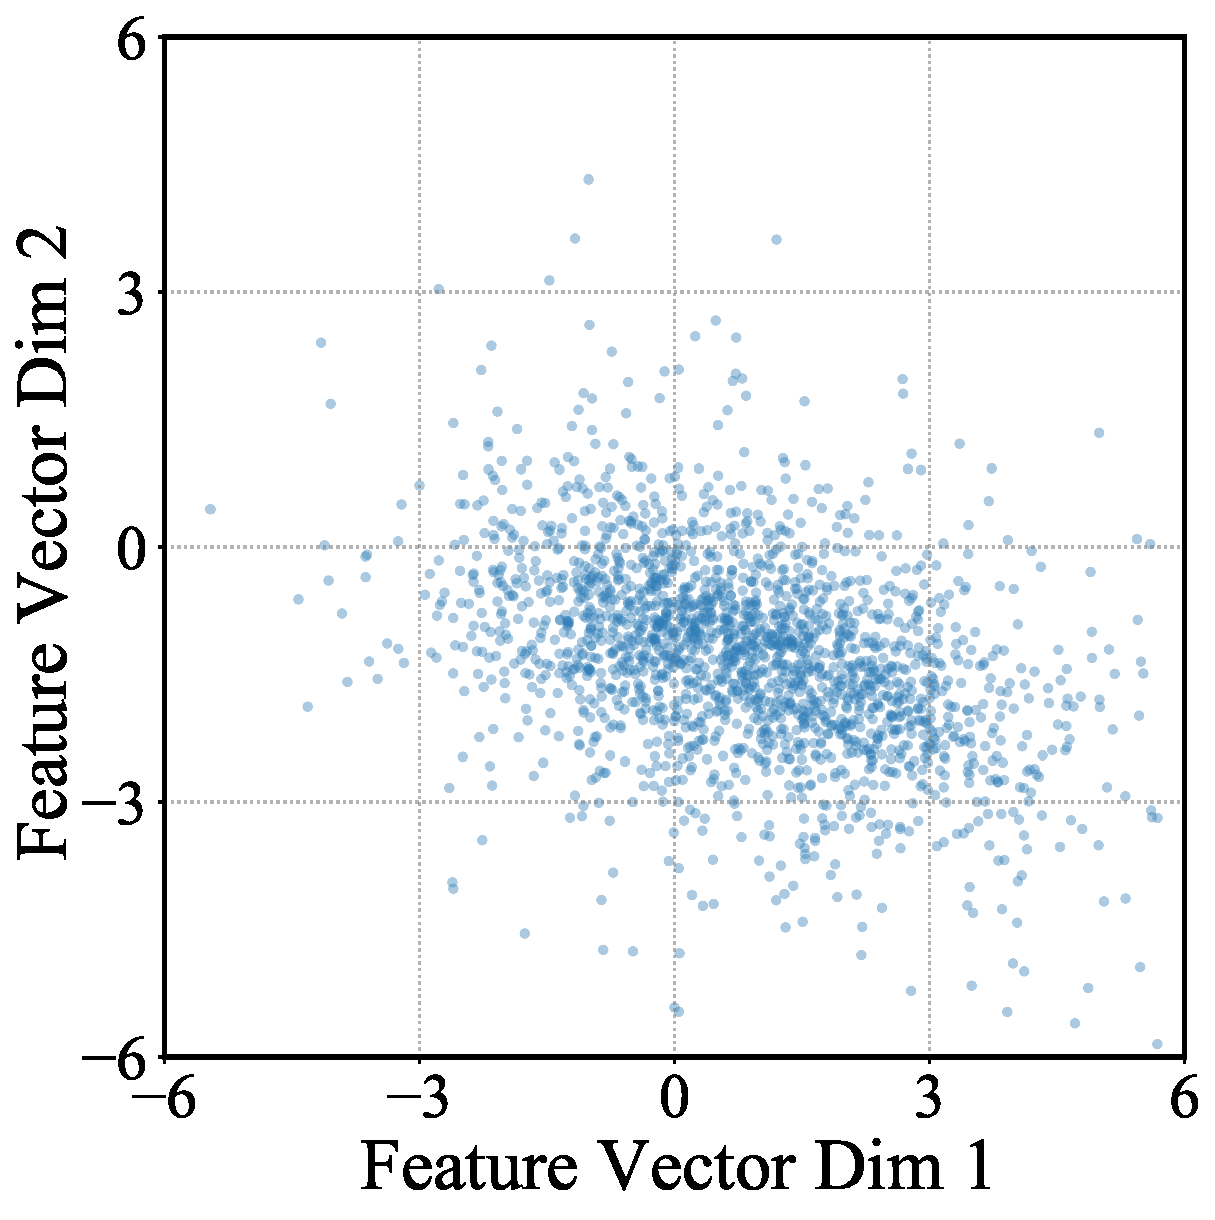
\includegraphics[width=0.24\textwidth]{figs/Gaussion/feature_visualization.pdf}
% 	}
%     \vspace{-2mm}
%     \caption{\small{Visualization of feature vectors.}}
%     \label{fig:gaussian assumptation}
%     \vspace{-8mm}
% \end{center}
% \end{figure} 

\begin{figure}[t]
    \centering
    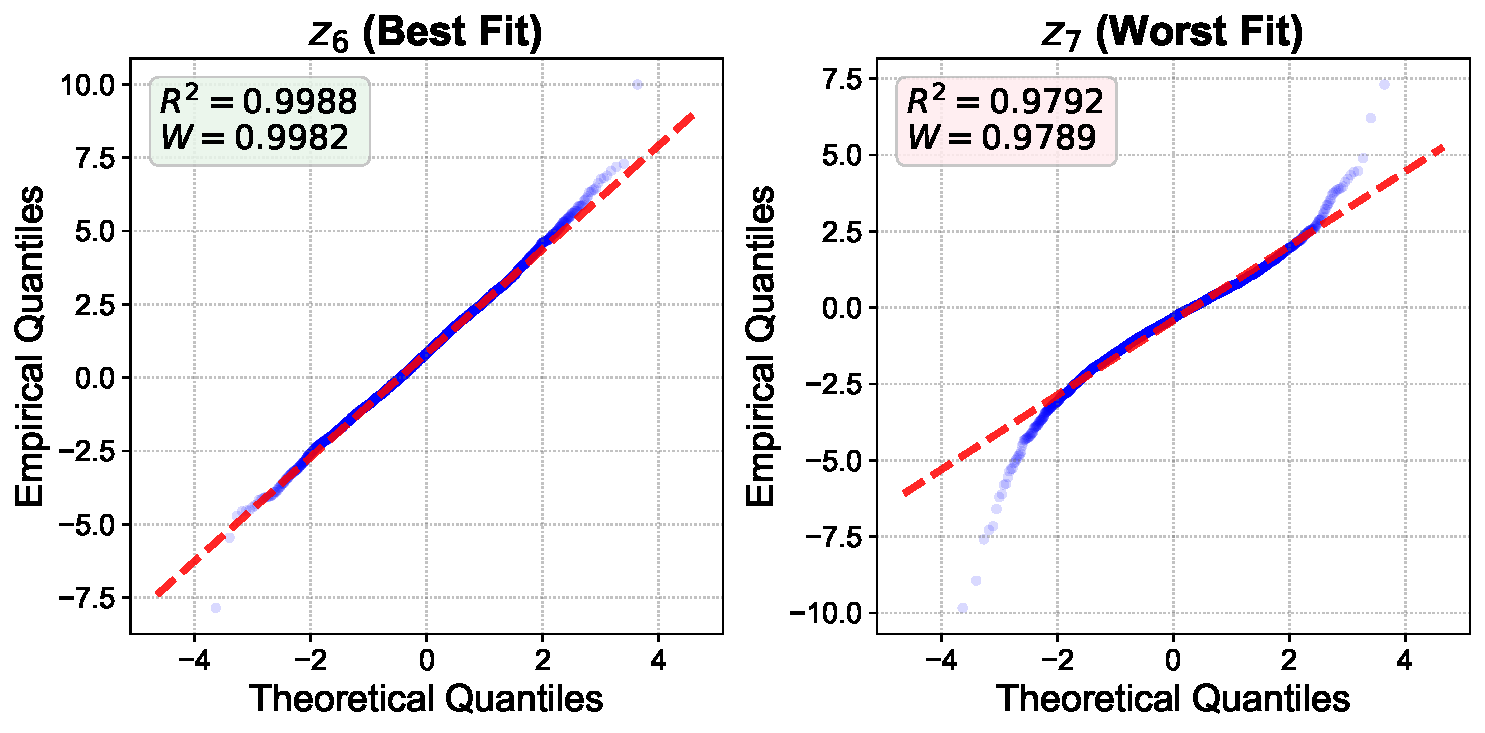
\includegraphics[width=\linewidth]{figs/Gaussion/qq_plots_1d_main.pdf} 
    \vspace{-6mm}
    \caption{\textbf{Gaussianity Validation via Q-Q Plots.} We visualize the feature dimensions with the highest $z_6$ (Left) and lowest ($z_7$, Right) conformance to the Gaussian hypothesis. \textbf{Note:} For visual clarity, plots display a random subset of 5,000 points, while the reported statistics ($R^2, W$) are computed on the \textbf{full validation set ($N=409,600$)}. The strong alignment with the red identity line ($y=x$) confirms that the learned features are predominantly Gaussian, with deviations confined to sparse heavy tails.}
    \label{fig:qq_main}
    \vspace{-4mm}
\end{figure}

% \paragraph{Gaussian Hypothesis Justification.} To justify the reasonableness of the Gaussian assumption, we extract feature vectors from the encoder and computed the density of arbitrary two dimensions by binning the data points into 29 groups, as visualized in Figure~\ref{fig:density}. Furthermore, we randomly selected 2000 data points from any two dimensions and plotted them in a scatter plot, as shown in Figure~\ref{fig:feature visualization}. It is evident that the feature vectors exhibit Gaussian-like characteristics. {\color{red} We also use Mahalanobis Distance~\citep{}, Results in Appendix~\ref{} show that while not perfectly normal, the majority of features
% closely approximate normal distributions, particularly in the central
% region where most samples lie. to be completed by Yuan.}
% %The underlying reason for this behavior can be attributed to the central limit theorem, which posits that learned feature vectors and code vectors will approximate a Gaussian distribution given a sufficiently large sample size and a relatively low-dimensional space, i.e., $d=8$.
% \vspace{-2ex}

% \paragraph{Gaussian Hypothesis Justification.} 
% To rigorously validate the Gaussian assumption underlying our Wasserstein objective, we conduct a statistical normality test on the learned latent features. Using the FFHQ dataset, we extract latent vectors from a subset of 1,600 images ($d=8$), yielding a large-scale sample size of $N=409,600$. Figure~\ref{fig:qq_main} visualizes the Quantile-Quantile (Q-Q) plots for the feature dimensions with the highest ($z_6$) and lowest ($z_7$) conformance to the Gaussian hypothesis. Ideally, if the feature distribution is Gaussian, the samples (blue points) should align strictly with the theoretical reference line (red dashed, $y=x$). As observed, the dimension with the best fit ($z_6$) exhibits near-perfect alignment with a coefficient of determination ($R^2$) of 0.9988. Crucially, even in the worst-case dimension ($z_7$), the bulk of the data closely adheres to the Gaussian profile ($R^2 > 0.979$), with deviations confined strictly to sparse heavy tails. This confirms that the learned features largely satisfy the Gaussian assumption, validating the theoretical foundation of our approach. We provide a comprehensive multivariate normality test using the Mahalanobis distance and full-dimension analysis in \textbf{Appendix~\ref{sec:normality_tests}}.

\paragraph{Gaussian Hypothesis Justification.} 
To empirically assess the Gaussian assumption underlying our Wasserstein objective, we analyze the distributional properties of the learned latent features. Using the FFHQ dataset, we extract latent vectors from a subset of 1,600 images ($d=8$), resulting in a total of $N=409{,}600$ samples. Figure~\ref{fig:qq_main} presents Quantile--Quantile (Q--Q) plots for the feature dimensions exhibiting the highest ($z_6$) and lowest ($z_7$) agreement with a Gaussian reference. Under an ideal Gaussian model, the samples (blue points) would align with the theoretical reference line (red dashed, $y=x$). As shown, the best-fitting dimension ($z_6$) demonstrates near-perfect alignment, with a coefficient of determination of $R^2 = 0.9988$. Importantly, even for the least-fitting dimension ($z_7$), the Q--Q plot over the full distribution achieves a high goodness-of-fit score ($R^2 > 0.979$). While mild deviations appear in the extreme tails, the central mass of the distribution remains well approximated by a Gaussian. These results indicate that the learned latent features are well modeled by a Gaussian distribution in the high-density region that dominates the probability mass, supporting the use of a Gaussian-based Wasserstein objective. A more comprehensive univariate and multivariate analysis, including Mahalanobis distance–based normality assessment across all dimensions, is provided in Appendix~\ref{sec:normality_tests}.
\vspace{-2ex}

\paragraph{Computational Overhead Analyses.} We evaluate the runtime efficiency of different VQ approaches by measuring the forward and backward pass times of the VQ module. As shown in Table~\ref{tab:computational overhead} in Appendix~\ref{appendix:computational overhead}, the runtime of Wasserstein VQ is only slightly longer than that of Vanilla VQ. This indicates that Wasserstein VQ maintains high computational efficiency, and that incorporating the quadratic Wasserstein distance does not incur a significant time overhead.
\vspace{-2ex}


\iffalse
\paragraph{Gaussian vs. Non-Gaussian Hypotheses.} We also consider Maximum Mean Discrepancy (MMD)~\citep{Gretton2012AKT, Sriperumbudur2009HilbertSE} as a more general alternative for distribution alignment. Unlike the Wasserstein-based approach, MMD operates in a Reproducing Kernel Hilbert Space (RKHS) without requiring explicit distributional assumptions. We denote this method as \emph{MMD VQ} and empirically compare it with \emph{Wasserstein VQ} on FFHQ. As shown in Table~\ref{tab:Gaussian Hypotheses} in Appendix~\ref{appendix:gaussian hypotheses}, MMD VQ achieves similar or slightly higher SSIM but shows no clear improvement in PSNR or reconstruction loss, suggesting that Gaussian versus non-Gaussian assumptions do not fundamentally affect codebook optimization.
\vspace{-2ex}
\fi

%\paragraph{Sensitivity Analysis on $\gamma$.} We perform sensitivity analysis on FFHQ dataset by varying $\gamma \in \{0, e^{-5}, e^{-4}, e^{-3}, e^{-2}, e^{-1}, e^{0}, e^{1}\}$, as shown in Table~\ref{tab:sensitivity analysis} in the Appendix~\ref{appendix:sensitivity analysis}, 

\paragraph{Additional Analyses.} Due to space limitations, further analyses are deferred to the appendix. Specifically, Appendix~\ref{appendix:representation visualize} visualizes the feature and code distributions across different VQ methods. Appendix~\ref{appendix:sensitivity analysis} presents a sensitivity analysis w.r.t. $\gamma$. Appendix~\ref{appendix:generalization ability} demonstrates that Wasserstein VQ exhibits strong generalization from ImageNet to FFHQ in terms of reconstruction performance. Finally, Appendix~\ref{appendix:ablation study} shows that Wasserstein VQ scales more effectively to larger codebooks ($K=100{,}000$) and higher feature dimensions (e.g., $d=32$).

%Due to space constraints, additional analyses are provided in the appendix. For example, in Appendix~\ref{appendix:representation visualize}, we visualize the feature and code distributions of different VQ methods.  In Appendix~\ref{appendix:sensitivity analysis}, we perform sensitivity analysis on $\gamma$. In Appendix~\ref{appendix:generalization ability}, \emph{Wasserstein VQ} shows strong generalization from ImageNet to FFHQ in reconstruction performance. In Appendix~\ref{appendix:ablation study}, we demonstrate that \emph{Wasserstein VQ} handles larger codebooks ($K=100{,}000$) and higher feature dimensions (e.g., $d=32$) more effectively.

%Due to space limitations, some additional analyses are provided in the appendix. For example,  in Appendix~\ref{appendix:representation visualize}, we visualize  Appendix~\ref{appendix:generalization ability}, \emph{Wasserstein VQ} demonstrates strong generalization from ImageNet to FFHQ in terms of reconstruction performance. In Appendix~\ref{appendix:ablation study}, we show that \emph{Wasserstein VQ} handles larger codebook sizes ($K=100{,}000$) and higher feature dimensions (e.g., $d=32$) more effectively.


\subsection{Evaluation on VQGAN Framework}
\paragraph{Dataset, Baselines, and Metrics.}
We evaluate our proposed method against a comprehensive set of baselines on the ImageNet and FFHQ datasets. For ImageNet, the compared methods include DQVAE~\citep{Huang2023TowardsAI}, DF-VQGAN~\citep{Ni2022NWALIPLI}, DiVAE~\citep{Shi2022DiVAEPI}, RQVAE~\citep{Lee2022AutoregressiveIG}, VQGAN~\citep{Esser2020TamingTF}, VQGAN-FC~\citep{Yu2021VectorquantizedIM}, VQGAN-EMA~\citep{Razavi2019GeneratingDH}, VQGAN-LC~\citep{Zhu2024ScalingTC}, Llama GEN~\citep{Sun2024AutoregressiveMB}, and VAR~\citep{Tian2024VisualAM}.
For FFHQ, we compare against RQVAE~\citep{Lee2022AutoregressiveIG}, VQGAN~\citep{Esser2020TamingTF}, VQGAN-FC~\citep{Yu2021VectorquantizedIM}, VQGAN-EMA~\citep{Razavi2019GeneratingDH}, VQ-WAE~\citep{Vuong2023VectorQW}, MQVAE~\citep{Huang2023NotAI}, and VQGAN-LC~\citep{Zhu2024ScalingTC}.

We adopt several widely used metrics to comprehensively evaluate visual reconstruction quality, including the Fréchet Inception Distance (r-FID)~\citep{Heusel2017GANsTB}, Reconstruction Inception Score (r-IS)~\citep{Salimans2016ImprovedTF}, Learned Perceptual Image Patch Similarity (LPIPS)~\citep{Zhang2018TheUE}, Peak Signal-to-Noise Ratio (PSNR), and Structural Similarity Index Measure (SSIM). Detailed descriptions of the experimental settings are provided in Appendix~\ref{appendix:experimental details}.
\vspace{-2ex}

\paragraph{Main Results.} As shown in Table~\ref{tab:reconstruction_IN-main table} and Table~\ref{tab:vqgan tranplant ffhq} in Appendix~\ref{appendix:supplement results on ffhq}, our proposed \emph{Wasserstein VQ} achieves the lowest r-FID within the VQGAN framework, demonstrating that VQ algorithms based on distribution matching can achieve superior reconstruction fidelity and perceptual quality. We further evaluate multi-scale quantization algorithms in Table~\ref{tab:reconstruction_IN-multi-scale}. Notably, all experiments in this table are fully controlled: the encoder–decoder architecture is identical to VAR~\citep{Tian2024VisualAM}, and, crucially, the latent features are kept fixed across all methods, ensuring that measurements of the criterion triple are unaffected by latent feature variance, as discussed in Appendix~\ref{appendix:Impact of Distribution Variance}. Under these controlled conditions, our \emph{Wasserstein VAR} achieves the best performance across the entire criterion triple, particularly yielding the lowest quantization error. Reconstruction performance further improves as we increase the number of decoder adaptation epochs, corresponding to stronger adversarial refinement; for example, for $K=8192$, the r-FID decreases steadily from \textbf{0.83} for Wasserstein VAR-a to \textbf{0.73} for Wasserstein VAR-c. Visualizations in Figures~\ref{fig:visual reconstruction ffhq} and~\ref{fig:visual reconstruction imagenet} (Appendix~\ref{appendix:reconstruction visualization}) show that the reconstructions produced by our approach remain nearly indistinguishable from the original inputs, confirming its strong visual tokenization capability.
\vspace{-1ex}



\section{Discussion of Distributional Matching Algorithms: MMD VQ vs. Wasserstein VQ}
\label{sec:discussion}